% WOCHAT 2026 / SIGDIAL-style 4-page submission manuscript.
% Canonical manuscript source for the local PDF artifact.
% For final EasyChair upload, paste this body into the official ACL/SIGDIAL
% template if WOCHAT publishes a required style file.
\documentclass[10pt,twocolumn]{article}

\usepackage[letterpaper,top=0.62in,bottom=0.70in,left=0.66in,right=0.66in]{geometry}
\usepackage{times}
\usepackage{latexsym}
\usepackage{microtype}
\usepackage{graphicx}
\usepackage{booktabs}
\usepackage{array}
\usepackage{url}
\usepackage[hidelinks]{hyperref}
\usepackage{xcolor}
\usepackage{caption}

\setlength{\columnsep}{0.23in}
\setlength{\parindent}{0.9em}
\setlength{\parskip}{0pt}
\setlength{\textfloatsep}{5pt plus 1pt minus 1pt}
\setlength{\floatsep}{5pt plus 1pt minus 1pt}
\setlength{\intextsep}{5pt plus 1pt minus 1pt}
\renewcommand{\baselinestretch}{0.94}
\captionsetup{font=small,skip=3pt}

\title{\vspace{-1.4em}
Are Agentic and Graph-Augmented RAG Worth It for Romanized Nepali Customer Support?\\
{\large A Controlled Evaluation across Three Synthetic Service Domains}}

\author{Sajak Basnet\\
Gomendra College\\
\texttt{sajak55460@gomendracollege.edu.np}}
\date{}

\begin{document}
\maketitle
\vspace{-1.6em}

\begin{abstract}
\noindent Retrieval-augmented generation (RAG) is attractive for customer-support dialogue because answers must be both conversational and grounded in policy. For low-resource, code-mixed settings such as Romanized Nepali, however, it is unclear whether complex agentic and graph-augmented RAG systems provide reliable gains over a controlled semantic baseline. We present a research-grade evaluation of traditional RAG, agentic RAG, and agentic GraphRAG on 300 matched Romanized Nepali customer-support queries across quick-commerce, cloud hosting, and digital wallet domains. The evaluation combines deterministic retrieval and operational metrics, GPT-5.2 LLM-as-judge scoring, stratified error analysis, paired bootstrap confidence intervals, paired permutation tests, Wilcoxon tests, and Holm--Bonferroni correction. Agentic GraphRAG obtains the highest mean overall score (0.7899), followed by agentic RAG (0.7894) and traditional RAG (0.7886), but the graph-over-traditional gain is only 0.0012, is not statistically significant, and is not practically meaningful. Traditional RAG is fastest and has the best quality-latency trade-off. The correct conclusion is that all three systems perform similarly under this benchmark; stronger graph- or agent-specific mechanisms are needed before claiming superiority for Romanized Nepali support RAG.
\end{abstract}

\section{Introduction}

Customer-support dialogue is a practical testbed for retrieval-augmented generation (RAG) \cite{lewis2020rag,gao2023rag}. A support assistant must answer in a helpful tone, respect company policy, decline unsupported actions, and expose the right escalation path. These requirements are sharper in Romanized Nepali, where customers frequently write informal transliterations, use flexible spellings, mix English service terms, and omit context. A query such as \emph{``mero order kata pugyo ani cancel garna milcha?''} is short, code-mixed, intent-rich, and company-specific. Retrieval must map it to the correct internal policy, while generation must not invent policy.

Recent RAG systems increasingly add query rewriting, routing, planning, tool use, memory, verification, and graph lookup. Such mechanisms are appealing because customer-support problems often contain hidden structure: accounts, orders, refunds, invoices, incidents, and escalation rules. Yet each added mechanism also increases latency, implementation cost, evaluation complexity, and failure surface. For an industry support system, a method should not be preferred merely because its mean score is slightly higher. The gain must be statistically reliable, practically meaningful, and justified against operational overhead.

This paper asks:
\begin{quote}
\emph{Do agentic RAG and agentic GraphRAG provide measurable advantages over traditional semantic RAG for Romanized Nepali customer support?}
\end{quote}
We answer with a controlled comparison over 300 matched queries and three synthetic company knowledge bases. The contributions are:
\begin{itemize}
\item a Romanized Nepali customer-support RAG benchmark spanning quick-commerce, cloud hosting, and digital wallet domains;
\item a modular evaluation pipeline combining retrieval metrics, LLM-as-judge generation metrics, robustness metrics, latency, and failure taxonomy;
\item paired statistical testing showing that the small observed advantage of GraphRAG is neither significant nor practically meaningful;
\item an industry-oriented interpretation of quality, latency, and deployment readiness.
\end{itemize}

\section{Benchmark and Systems}

\paragraph{Dataset.}
The dataset contains 300 Romanized Nepali and code-mixed Nepali-English support queries, with 100 queries per company. The companies are a quick-commerce/e-commerce provider, a hosting/cloud provider, and a FinTech/digital wallet provider. Each query includes a query identifier, company label, difficulty label, category or intent, and the user query text. The difficulty split contains simple FAQ-style questions, medium procedural questions, and complex multi-constraint or ambiguous questions. This design tests both direct retrieval and harder support behavior such as escalation, policy boundary handling, and multi-step reasoning.

\paragraph{Knowledge bases.}
Each company has an internal Markdown knowledge base covering policy, support tone, operational procedures, incident handling, and escalation rules. Documents are chunked deterministically and indexed in company-specific vector collections. During evaluation, the query's company label selects the corresponding knowledge base, preventing accidental comparison across different domains while still allowing detection of cross-company contamination in retrieved evidence.

\paragraph{Architectures.}
The comparison includes three architecture slots. Traditional RAG embeds the query, retrieves top-$k$ chunks from the selected company collection, and generates an answer from the retrieved context. Agentic RAG represents an agent-enabled architecture slot with a separate output stream and evaluation label. Agentic GraphRAG represents a graph-augmented slot intended to test whether structured retrieval improves support answers. In this controlled run, all systems are evaluated from their existing saved outputs; no system is rerun during analysis, and all comparisons are matched by query ID.

\section{Evaluation Methodology}

\paragraph{Metrics.}
The evaluator computes retrieval, generation, Romanized Nepali robustness, and operational metrics. Retrieval metrics include context precision, context recall, context relevancy, hit rate@$k$, MRR@$k$, nDCG@$k$, average retrieved chunks, empty retrieval rate, duplicate chunk rate, and cross-company contamination. Generation metrics include faithfulness or groundedness, answer relevancy, correctness, completeness, hallucination rate, and policy compliance. Robustness metrics include romanized query understanding, code-mixed handling, intent classification accuracy, company-domain accuracy, escalation correctness, and tone appropriateness. Operational metrics include success rate, failure rate, mean latency, median latency, p95 latency, and p99 latency. Missing telemetry such as token usage or true tool-call counts is reported as unavailable rather than fabricated.

\paragraph{LLM-as-judge.}
GPT-5.2 is used as the judge for faithfulness, answer relevancy, answer correctness, completeness, policy compliance, Romanized query understanding, and tone. The judge receives the query, generated answer, retrieved context, and available expected topic/source metadata. LLM-as-judge methods are useful for scalable NLG evaluation \cite{liu2023geval,kocmi2023large,guo2023close}, but they may encode model-specific preferences. We therefore treat judge scores as one evidence source and combine them with deterministic retrieval checks, latency metrics, and paired statistical tests.

\paragraph{Statistical testing.}
Because all architectures answer the same 300 query IDs, the correct tests are paired. We compute bootstrap confidence intervals over per-query means, paired bootstrap confidence intervals for architecture differences, paired permutation tests, Wilcoxon signed-rank tests when available, Cohen's $d_z$, Cliff's delta, and Holm--Bonferroni adjusted $p$-values \cite{efron1994bootstrap,demsar2006statistical}. A difference below 0.01 on the normalized overall score is treated as not practically meaningful, even if statistically detectable.

\section{Overall Results}

\begin{table}[t]
\centering
\small
\begin{tabular}{lrrrr}
\toprule
Architecture & Mean & 95\% CI & Median & Std. \\
\midrule
Traditional RAG & 0.7886 & [0.7759, 0.8014] & 0.8157 & 0.1103 \\
Agentic RAG & 0.7894 & [0.7769, 0.8019] & 0.8158 & 0.1095 \\
Agentic GraphRAG & \textbf{0.7899} & [0.7774, 0.8025] & 0.8186 & 0.1096 \\
\bottomrule
\end{tabular}
\caption{Overall GPT-5.2 judged composite scores. Confidence intervals overlap almost completely.}
\label{tab:overall}
\end{table}

Table~\ref{tab:overall} shows a very small ranking difference. Agentic GraphRAG has the highest mean score, but the absolute gain over traditional RAG is 0.0012. The standard deviations are nearly identical, and the confidence intervals almost fully overlap. This already suggests that the ranking should be interpreted cautiously rather than as evidence of a decisive architecture improvement.

\begin{table}[t]
\centering
\small
\begin{tabular}{lrrrr}
\toprule
Comparison & Diff. & 95\% CI & Holm $p$ & $d_z$ \\
\midrule
Trad. $-$ Agentic & -0.0007 & [-0.0031, 0.0016] & 1.0000 & -0.0366 \\
Trad. $-$ Graph & -0.0012 & [-0.0036, 0.0012] & 0.9635 & -0.0580 \\
Agentic $-$ Graph & -0.0005 & [-0.0028, 0.0019] & 1.0000 & -0.0238 \\
\bottomrule
\end{tabular}
\caption{Paired significance tests on overall score. All corrected comparisons are non-significant, and all effect sizes are negligible.}
\label{tab:significance}
\end{table}

Table~\ref{tab:significance} gives the main statistical result. Every paired confidence interval crosses zero, every Holm-corrected $p$-value is non-significant at $\alpha=0.05$, and the paired effect sizes are negligible. Therefore, the correct research claim is not that GraphRAG is better, but that the evaluated systems are closely matched on this dataset.

\section{Stratified Analysis}

\begin{table}[t]
\centering
\small
\begin{tabular}{lllrr}
\toprule
Group & Best & Score & Lat. & Note \\
\midrule
Hosting/cloud & Agentic & 0.7839 & 2722 & tied \\
Wallet/FinTech & Graph & 0.7528 & 2898 & tied \\
Quick-commerce & Agentic & 0.8337 & 2588 & tied \\
Simple & Agentic & 0.8157 & 2768 & tied \\
Medium & Graph & 0.8058 & 4474 & tied \\
Complex & Traditional & 0.7411 & 2650 & tied \\
\bottomrule
\end{tabular}
\caption{Best mean score by company and difficulty. All observed wins are practical ties. Latency is mean milliseconds for the listed architecture.}
\label{tab:strata}
\end{table}

Stratification avoids hiding domain-specific behavior. On hosting/cloud and quick-commerce, agentic RAG is marginally highest. On the wallet domain, GraphRAG is marginally highest. By difficulty, agentic RAG is marginally highest on simple queries, GraphRAG on medium queries, and traditional RAG on complex queries. None of these differences is large enough to support a strong subgroup claim. Importantly, GraphRAG does not show a complex-query advantage: complex-query means are 0.7411 for traditional RAG, 0.7409 for GraphRAG, and 0.7405 for agentic RAG. If graph retrieval is expected to help multi-hop or complex cases, this implementation has not yet demonstrated that benefit.

\begin{figure}[t]
\centering
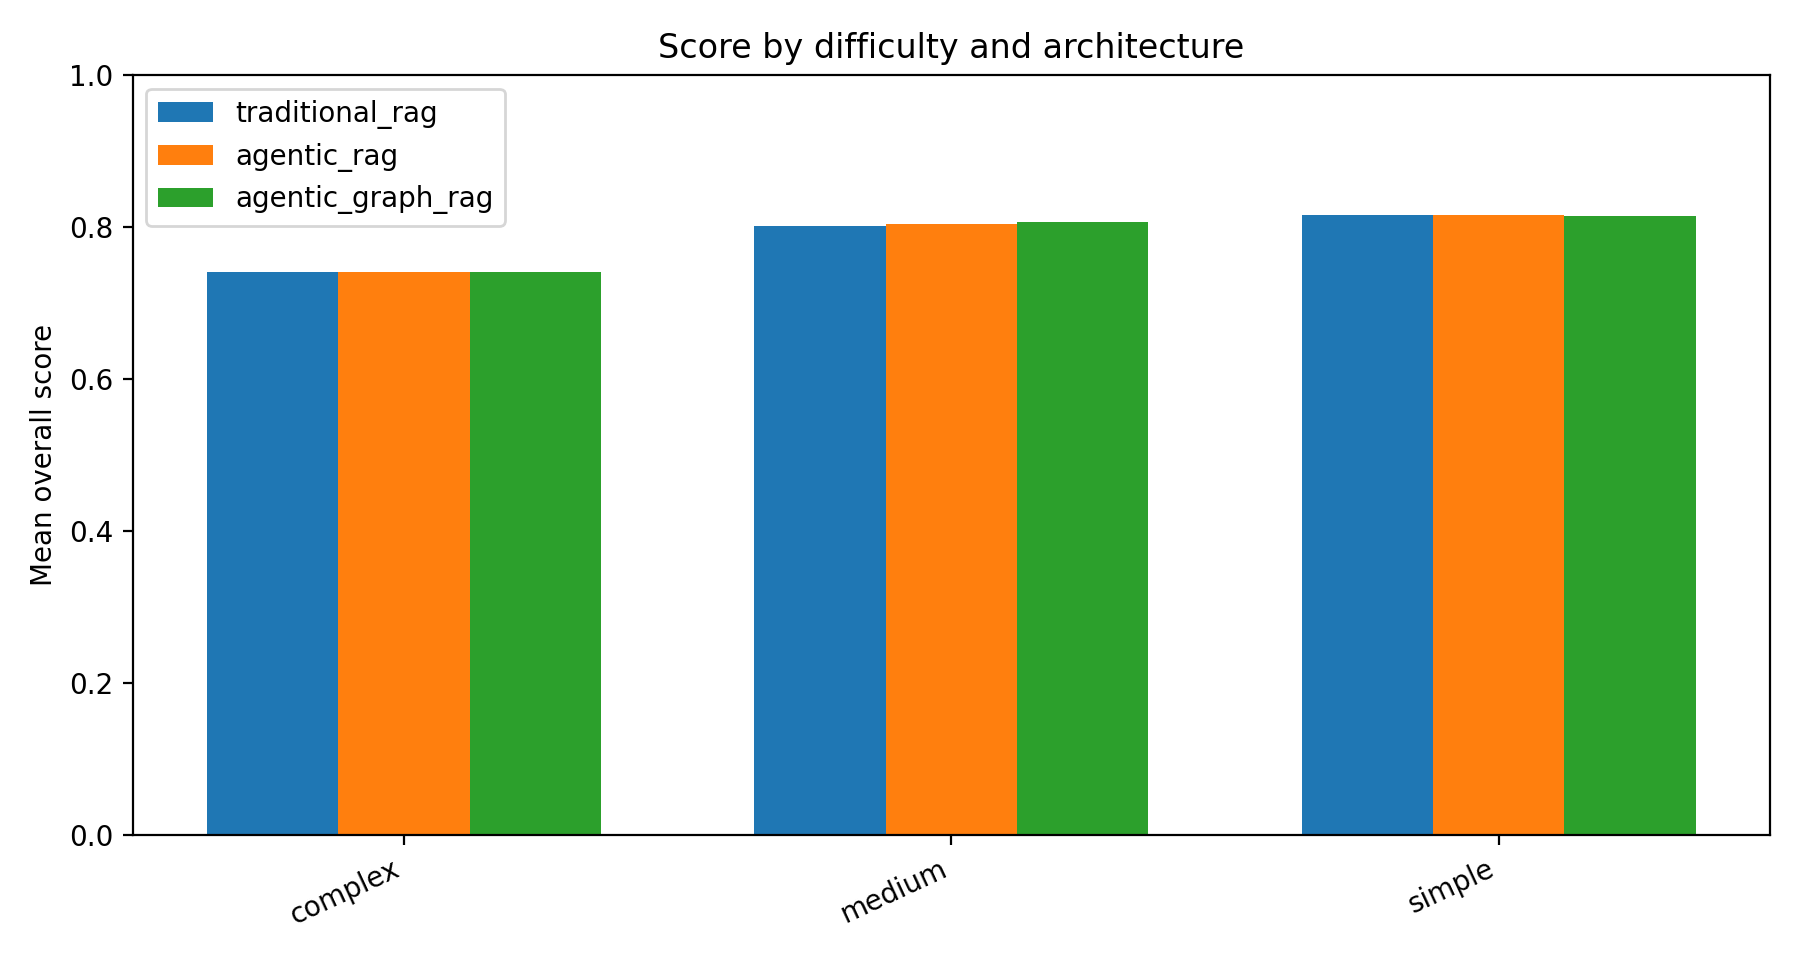
\includegraphics[width=\columnwidth]{../results/analysis/figures/score_by_difficulty_architecture.png}
\caption{Mean overall score by difficulty and architecture. The systems remain tightly clustered across difficulty levels.}
\label{fig:difficulty}
\end{figure}

\begin{figure}[t]
\centering
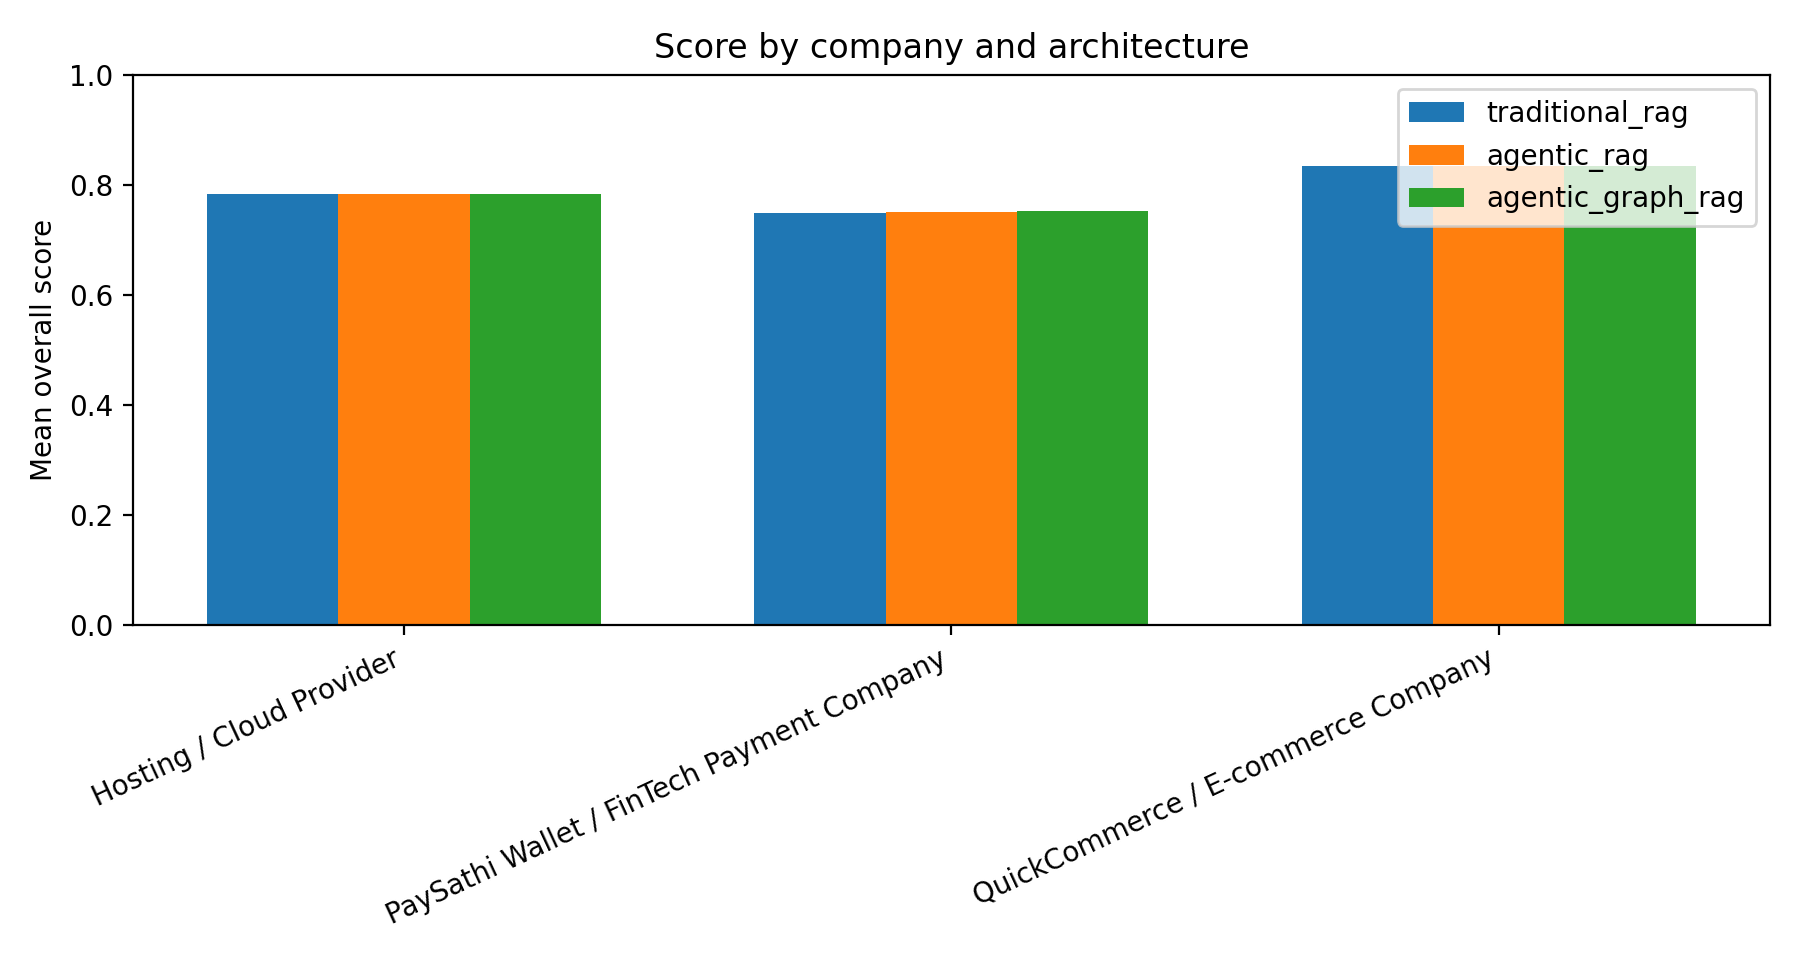
\includegraphics[width=\columnwidth]{../results/analysis/figures/score_by_company_architecture.png}
\caption{Mean overall score by company and architecture. No company has a practically decisive architecture winner.}
\label{fig:company}
\end{figure}

\section{Retrieval, Latency, and Efficiency}

\begin{table}[t]
\centering
\small
\begin{tabular}{lrrrr}
\toprule
Architecture & Recall & Hit@$k$ & MRR & Chunks \\
\midrule
Traditional RAG & 0.7400 & 0.7400 & 0.6178 & 4.0 \\
Agentic RAG & 0.7400 & 0.7400 & 0.6178 & 4.0 \\
GraphRAG & 0.7400 & 0.7400 & 0.6178 & 4.0 \\
\bottomrule
\end{tabular}
\caption{Retrieval metrics are identical across systems in this run.}
\label{tab:retrieval}
\end{table}

Retrieval behavior explains much of the outcome. All three systems retrieve four chunks on average and have identical context recall, hit rate@$k$, and MRR@$k$. The analysis detects no empty retrieval and no cross-company contamination. Retrieval quality correlates strongly with final answer score (about 0.83 for all systems), implying that better evidence selection is likely more valuable than orchestration unless the orchestration actually changes evidence quality.

\begin{table}[t]
\centering
\small
\begin{tabular}{lrrrr}
\toprule
Architecture & Mean ms & p95 ms & Gain & Gain/sec \\
\midrule
Traditional RAG & \textbf{2524} & \textbf{3510} & -- & -- \\
Agentic RAG & 2637 & 3548 & 0.0007 & 0.0065 \\
GraphRAG & 3099 & 3570 & 0.0012 & 0.0021 \\
\bottomrule
\end{tabular}
\caption{Quality-latency trade-off relative to traditional RAG.}
\label{tab:latency}
\end{table}

Latency changes the deployment interpretation. Traditional RAG is fastest. Agentic RAG adds 113 ms for a 0.0007 quality gain. GraphRAG adds 575 ms for a 0.0012 quality gain. These ratios do not justify a production switch under the current evidence. For an industry system, traditional RAG is the most production-ready choice because it is simpler, fastest, and statistically tied in quality.

\begin{figure}[t]
\centering
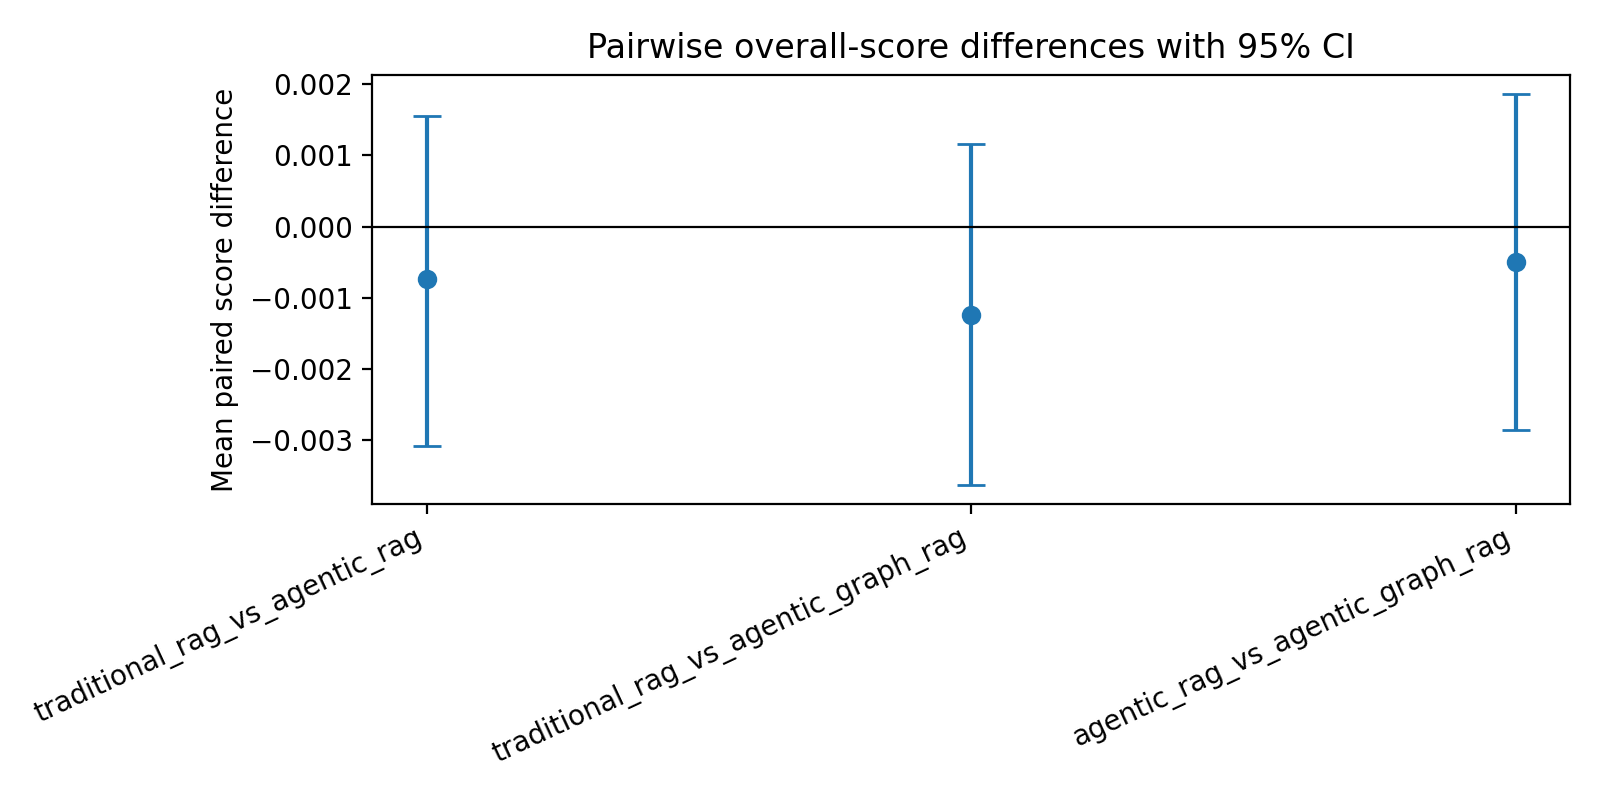
\includegraphics[width=\columnwidth]{../results/analysis/figures/pairwise_score_difference_plot.png}
\caption{Paired score differences with confidence intervals. Intervals crossing zero prevent a superiority claim.}
\label{fig:diff}
\end{figure}

\section{Failure Analysis}

Failure counts are low overall, but the taxonomy clarifies where future work should focus. Traditional RAG has 17 retrieval-miss flags, 17 partial-answer flags, and 14 hallucinated-policy flags. Agentic RAG has 14, 14, and 13 respectively. GraphRAG has 12, 12, and 12 respectively, but also 5 cases labeled as latency overhead without quality gain. No architecture shows wrong-company policy contamination. The dominant pattern is evidence mismatch followed by incomplete or unsupported policy advice, which is consistent with known hallucination risks in grounded generation \cite{ji2023hallucination}.

Representative low-scoring examples show that failures are rarely caused by Nepali surface form alone. More often, the answer misses a policy condition, gives a partially correct escalation path, or answers confidently when the retrieved context is incomplete. This suggests that the next useful improvement is not simply a larger orchestration layer, but denser gold supervision for expected source documents, expected answer points, and ambiguity handling.

\section{Practical Interpretation}

For an industry deployment, the fastest statistically tied model is usually the better default. Traditional RAG has the simplest operational path: fewer moving parts, lower mean latency, lower tail latency, and no observed quality disadvantage after paired testing. Agentic RAG remains useful as an experimentation layer when future runs add real planning, clarification, tool use, or verification behavior. GraphRAG is most promising as a research direction if it changes evidence selection, reduces retrieval misses, or improves complex-query handling rather than only adding orchestration overhead.

For a research claim, the strongest result is negative but useful: under controlled retrieval, additional architecture labels do not automatically create measurable gains in Romanized Nepali customer support. This discourages architecture inflation and emphasizes matched-query evaluation, confidence intervals, multiple-comparison correction, and latency-aware interpretation.

\section{Threats to Validity}

The benchmark uses synthetic companies and synthetic queries, so real production traffic may expose different ambiguity, spelling, and adversarial patterns. GPT-5.2 judge scores may reflect judge-model preferences despite deterministic checks. Gold answer points and expected source documents are incomplete for some queries, increasing reliance on judge scoring. The current agentic and graph-labeled outputs share much of the retrieval surface with the baseline, limiting the opportunity for large retrieval differences. Finally, a different composite weighting could shift very small rankings, although it is unlikely to make a 0.0012 gain practically meaningful.

\section{Conclusion}

Agentic GraphRAG has the highest mean score, but the advantage is not statistically significant and not practically meaningful. The graph-over-traditional mean gain is 0.0012, the paired confidence interval crosses zero, and the Holm-adjusted permutation $p$-value is 0.9635. Traditional RAG is fastest and has the best quality-latency trade-off. Simple, medium, and complex query strata all show practical ties rather than a stable architecture winner.

The final research claim should therefore be conservative and credible: \emph{on this Romanized Nepali customer-support benchmark, traditional RAG, agentic RAG, and agentic GraphRAG perform similarly; the current evidence does not justify claiming that agentic or graph-augmented RAG is superior to a controlled semantic baseline.} The next experiment should add human-authored gold answer points, expected source documents for every query, real user traffic, and telemetry for token cost, tool calls, graph hops, and agent steps. Only then can graph and agentic mechanisms be evaluated as mechanisms rather than labels.

\section{Recommendations for the Next Experiment}

The next benchmark version should separate mechanism from label. A true agentic condition should log planning steps, clarification decisions, tool calls, verifier decisions, and fallback behavior. A true graph condition should log entity linking, graph hops, relation types, and whether graph-selected evidence differs from vector-selected evidence. Without this telemetry, it is difficult to explain why a method wins or loses.

The dataset should also add complete expected answer points and expected source documents for every query. This would allow stronger deterministic scoring of source coverage, contradiction, and missing policy conditions. A small human review set should calibrate the LLM judge, especially for Romanized Nepali tone, ambiguity handling, and code-mixed intent. Finally, the production comparison should include cost per query, p99 latency, rate-limit behavior, and human handoff accuracy.

\section*{Ethics and Artifact Availability}

The benchmark is synthetic and does not contain private customer messages, account identifiers, payment credentials, or real support transcripts. This lowers privacy risk but also limits ecological validity. Any future deployment study should use consented or properly anonymized data and include human review for sensitive financial and hosting decisions.

The benchmark should not be interpreted as a production chatbot release. It is an evaluation artifact for studying retrieval, grounding, code-mixed language handling, and architecture trade-offs. All generated analysis files, detailed metric JSONL outputs, figures, and the paper-generation script are stored in the repository so reviewers can inspect per-query scores, validation summaries, significance tests, failure taxonomy, and chart data.

\section*{Reproducibility}
\small
All result files are stored under \texttt{results/}. The analysis report and figures are generated with:
\begin{quote}
\texttt{uv run python -m ragbench.analysis.research\_grade\_eval --results-dir results --output-dir results/analysis --bootstrap-samples 10000 --alpha 0.05}
\end{quote}

\bibliographystyle{plain}
\bibliography{references}

\end{document}
